% 2019-09-16
%
% Header can be about me and past tense: I have done X Y Z
%
% Body should describe results in the present tense, normal technical style
%
% The end of a section may use self-cites, and those may use past tense to
%  say "I did ...."

My research to date has focused on
 understanding the performance challenges for natural
 and comparing natural to other approaches.
These efforts have led up to the above thesis question.
The performance studies motivate a combination of \tdeep{} and \tshallow{}
 types, and suggest methods to empirically validate the result.
The comparison studies provide a theoretical model for defining the
 combination and understanding its formal guarantees.

% others = their they
%
% mine = our we

% This section reviews my prior work and explains how each project contributes
%  to the thesis question.


\subsection{Performance Evaluation}

Migratory typing promises the ability to mix typed and untyped code.
A performance evaluation for a migratory typing system must, therefore,
 evaluate mixed-typed programs.\footnote{\shorturl{https://www.}{ccs.neu.edu/home/asumu/papers/stop15-tfgnvf.pdf}}

\citet{tfdfftf-ecoop-2015} present the first systematic evaluation
 of a mixed-typed language.
The paper applies a method to two fully-typed programs consisting of four
 modules; for each program, this method demands the generation and
 measurement of $2^4$ partially-typed configurations.
The paper tabulates the results of this evaluation in two lattices showing
 the fully-untyped configuration on the bottom and fully-typed on top
 (\figureref{fig:takikawa-lattice}),
 and thereby shows the running times a programmer
 might see if they added the same types in an arbitrary manner.
Using these lattices, the paper discusses the worst-case performance
 and the existence of bottom-up paths through the lattice that avoid slowdowns.

\begin{figure}[h]
  \begin{tabular}{c@{\qquad\qquad}c}
  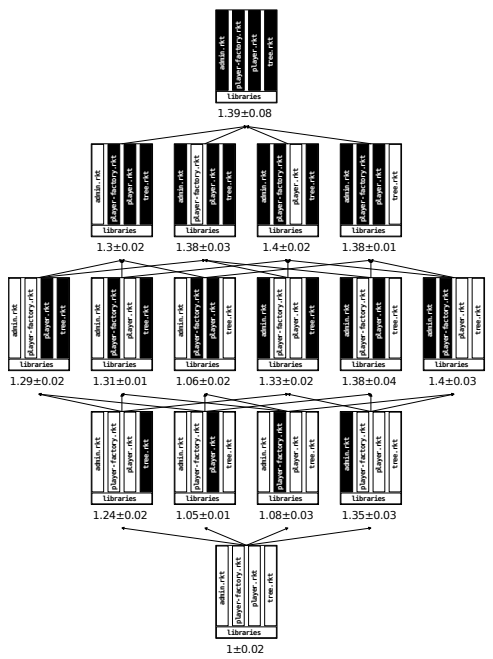
\includegraphics[width=0.30\columnwidth]{src/takikawa-lattice-acquire.png}
    &
  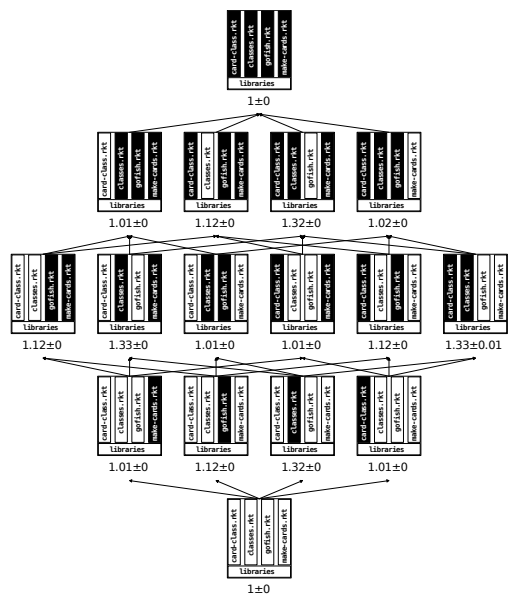
\includegraphics[width=0.30\columnwidth]{src/takikawa-lattice-gofish.png}
  \end{tabular}
  \caption{Performance results for two Typed Racket programs~\cite{{tfdfftf-ecoop-2015}}}
  \label{fig:takikawa-lattice}
\end{figure}

The method clearly needs further refinement; a lattice presents a lot
 of information, but does little to convey insights.
Furthermore, the exhaustive approach to data collection cannot handle large
 programs.
To summarize, the method raises at least three questions of size and scale:
 \begin{itemize}
   \item Is there a concise way to summarize the performance of a program?
   \item Can the method compare different implementations of migratory typing?
   \item Can the method be adapted to programs with a large number (+20) of configurations?
 \end{itemize}
My work on performance evaluation developed answers to these questions.


\subsubsection{Summarizing Performance}
% D-deliverable

Turing's negative answer to the halting problem tells us that a computer
 program cannot tell the difference between an infinite running time and
 a very large one.
This suggests a corresponding law for software developers:
 all programs that are not ``fast enough'' are equally worthless.

\citet{tfgnvf-popl-2016} use this relevance law to summarize the performance
 of a migratory typing system.
If a configuration is fast enough, then it is good.
Otherwise it is worthless.
In this way, a performance lattice defines a ratio; namely, the proportion of
 good configurations.
A software developer can examine the ratios for a set of benchmarks to
 assess the performance risk of migratory typing for their own code.

Technically, \citet{tfgnvf-popl-2016} call a configuration \deliverable{D}
 if its running time is no more than $D$x slower than a baseline running
 time.\footnote{One useful baseline is the performance of the host language
 with absolutely no migratory typing.
 (This may differ from the fully-untyped configuration in a lattice~\cite{gm-pepm-2018}.)
 Other baselines may prove useful in the future.}
Given a positive value for $D$, the proportion of \deliverable{D} configurations
 is the proportion of ``good'' configurations.
They accommodate varying notions of good performance by combining the results
 for $D$ between $1$ and $20$ in a plot

 CDF ...


To accommodate varying requirments, they present the 

They accommodate varying performance requirements by reporting the percent
 of \deliverable{D} configurations for $D$ ranging between 1 and 20.
 


Given a parameter $D$ 

Given a parameter $D$




In 2015, \citet{tfdfftf-ecoop-2015} measured the performance impact of gradual typing on
 two object-oriented programs.
Their key insight was to begin with a fully-typed program and measure the
 running time of all gradually-typed configurations obtained by removing
 some type annotations.
By working backwards from the types, the method lets a researcher systematically
 visit the codes that a programmer may encounter as they migrate an
 application.
By measuring all configurations, the method enables general claims about
 migratory typing---which, after all, advertises the freedom to mix typed
 and untyped code.

This method for collecting data motivated a larger study.
I helped develop (and measure) 12 functional benchmark programs, ranging in
 size from 30 to 6,000 lines of code, for an evaluation of Typed
 Racket~\cite{tfgnvf-popl-2016}.

During the evaluation, it became clear that the data analysis was a major
 issue.
The first evaluation~\cite{tfdfftf-ecoop-2015} had studied two program of four modules each
 and presented the results in two powerset lattices of $2^4$ configurations.
This visualization method was impractical for programs with seven or more
 module.
The typical ``summary statistics'' of mean, median, min, and max were also a
 poor fit; although worst-case performance could be terrible
 (\figureref{fig:max-overhead}), there is no guarantee that a programmer
 will actually encounter the worst case.

To summarize our exponentially-large datasets, we formulated the notion
 of a \deliverable{D} configuration.
A mixed-typed configuration is \deliverable{D} if it runs at most $D$ times
 slower than a fully-untyped baseline configuration.
For programmers, the relevant question is what percent of all configurations
 are \deliverable{D} for a few critical values.
If a team is willing to accept a 6x slowdown due to migratory typing,
 and the percent of \deliverable{6} configurations is above 90\% on a suite
 of representative benchmarks, then they may conclude that new types are
 unlikely to break their performance goal.

Our 2016 paper~\cite{tfgnvf-popl-2016} plots the proportion of
 \deliverable{D} configurations for $D$ between 1x and 20x.
The results gave an extremely negative image of natural-style migratory typing;
 in half the benchmarks, fewer than 60\% of all configurations were
 \deliverable{20}.
The plots also explored whether adding types to two additional modules could
 improve performance in the best case.
Unfortunately, the extra conversions steps could not guarantee a drastic
 performance improvement.
For example, the plots in \figureref{fig:snake-popl} show the percent of
 \deliverable{D} configurations allowing 0, 1, and 2 extra conversion steps.
Even in the rightmost plot, allowing 2 angelic conversion steps, there are
 still many (~20\%) configurations that run 10 times slower than the baseline.

\begin{figure}[h]
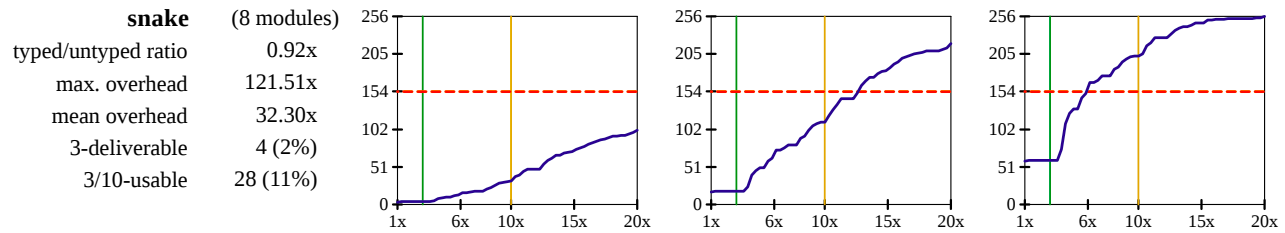
\includegraphics[width=0.96\columnwidth]{src/snake-popl.png}
\caption{Counting \deliverable{D} configurations in the \bm{snake}
         benchmark~\cite{tfgnvf-popl-2016}. The $x$-axis ranges over $D$ values;
         the vertical lines mark $D=3$ and $D=10$.
         The $y$-axis counts configurations; the dashed horizontal line marks
         $60$\% of all configs.
         The thick blue line is the number of \deliverable{x} configs.}
\label{fig:snake-popl}
\end{figure}


\subsubsection{Comparing Implementations}

The evaluation of Typed Racket inspired many efforts to improve its performance.
Sam Tobin-Hochstadt fixed issues in Typed Racket and modified it to produce
 simpler contracts for common function shapes.
Robert Bruce Findler greatly reduced the allocation costs of Racket contracts.
Others, including myself, contributed smaller patches.

All told, Typed Racket changed significantly between versions 6.2 (June 2015)
 and 6.4 (February 2016).
The evaluation method quantified the effect of these changes on
 performance with plot containing multiple \deliverable{D} curves on the same
 axis~\cite{gtnffvf-jfp-2019}.
To demonstrate, \figureref{fig:snake-jfp} presents curves for the \bm{snake}
 benchmark on Racket 6.2, 6.3, and 6.4.
The curve for version 6.4 lies above the others, meaning the percent of
 \deliverable{D} configurations is increased for every value of $D$ along
 the $x$ axis.

\begin{figure}[h]
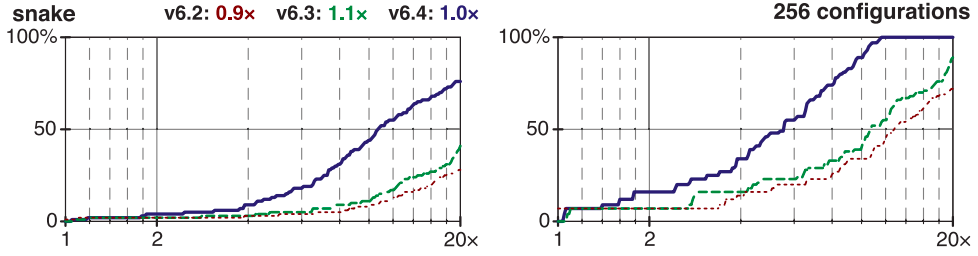
\includegraphics[width=0.8\columnwidth]{src/snake-jfp.png}
\caption{Comparing performance across three versions of Typed Racket}
\label{fig:snake-jfp}
\end{figure}

\citet{fgsfs-oopsla-2018} later contributed a major change to the contract system:
 collapsible higher-order contracts.
Once again, the exhaustive evaluation method was one of the ways that we
 measured the impact of the new contracts.


\subsubsection{Scaling the Method}

Concurrently with the improvements to Typed Racket, Zeina Migeed and I
 adapted the evaluation method to Transient Reticulated Python~\cite{gm-pepm-2018}.
This proved challenging because Reticulated allows type annotations
 at a finer granularity than Typed Racket; in particular, any function
 parameter, function return, and class field may have a type annotation.
Additionally, Reticulated changes the behavior of untyped Python code that
 it preprocesses.

For our evaluation, we elected to type entire function and class definitions
 as one ``unit'' of type conversion.
We also added one configuration to the space, with Python running the untyped
 code, as a baseline for comparisons.
In a program with three functions and four classes, we thus explored
 $2^{3+4} + 1$ configurations for the evaluation.

Even this coarse space, however, is too large to evaluate programs with more
 than $20$ functions and classes.
To overcome this practical limitation, we developed a method based on
 simple random sampling to approximate the number of \deliverable{D}
 configurations in a benchmark.
The sampling method counts the percent of \deliverable{D} configurations
 in a few sets of configurations, whose members are chosen uniform-randomly;
 the resulting set of percentages provides a confidence bound for the true
 percent of \deliverable{D} configurations.

We validated the sampling method on six benchmarks with $12$ to $17$ ``unit''
 of type conversion each (consequently, $2^{12}$ to $2^{17}$ configurations).
For each of these benchmarks, we conducted both an exhaustive evaluation and
 an approximate one; the approximation took $10$ samples with $120$ to $170$
 configurations in each sample.
The $95$\% confidence intervals for the samples yielded tight bounds on the
 true percents of \deliverable{D} configurations for $D$ between $1$x and
 $10$x.
Therefore, we conclude that the method is useful for benchmarks in which we
 cannot obtain ground-truth results in a practical timeframe.


\subsection{Comparative Models}

Models of migratory typing systems come in many varieties---often because
 the models reflect a proof-of-concept implementation~\cite{bat-ecoop-2014,wnlov-popl-2010,mt-oopsla-2017,vss-popl-2017,tf-popl-2008}.
 % TODO cite many more
These models share the common goal of mixing static and dynamic typing,
 but realize the goal with different formalizations.
Unfortunately, the lack of a common model makes it difficult to compare the
 properties satisfied by each.

\citet{clzv-ecoop-2018} address the diversity with a typed language, \kafka{},
 that can express different methods of enforcing types.
The paper uses \kafka{} as a target language for four translations from
 a mixed-typed surface language; the translations represent natural,
 concrete, erasure, and transient.
The paper illustrates the different semantics with examples, but does not
 provide a formal characterization.

For my work on comparing styles of migratory typing, we developed
 a model that expresses styles as different semantics
 for a common surface language.
The common model enabled fair comparisons of properties
 such as type soundness and complete monitoring.
Additionally, the model encouraged the design of new semantics for migratory
 typing.
% Need to mention other things? This paragraph should lead into the subsections

\subsubsection{Apples to Apples Comparison}

% developed model, (1) what are boundaries (2) what are checks
% implemented for TR
% - same method! aha
% - 

Building on the \citet{mf-toplas-2009} multi-language approach, we designed
 a model of a mixed-typed language.
The model combines a typical statically-typed language and an independent
 dynamically-typed language.
Every mixed-typed program in the model links components from the sub-languages
 with boundary expressions.
These boundaries are the initial channels of communication between typed and
 untyped code.
During evaluation new channels may arise, but the models keep a separation
 between the two languages.

The main question for a semantics is what to do when a value crosses one
 of the boundaries separating typed and untyped code.
Natural eagerly and deeply checks values if possible, and otherwise wraps
 an incoming higher-order value in a proxy wrapper.
If a wrapped value is later used, the wrapper checks its behavior against
 the boundary type.
Transient performs type-tag checks at boundaries, but additionally
 treats every elimination form in typed code as a potential boundary.
These shallow checks match a value against the shape expected by the
 client context; they do not fully enforce the types at the boundaries.

% more to say? surely

\begin{figure}[h]
  \(\begin{array}[t]{l@{\qquad}l}

  \fbox{$\DNsym : \tpair{\stype}{\svalue} \rightarrow \svalue \cup \serror$}
  &
  \fbox{$\SNsym : \tpair{\stype}{\svalue} \rightarrow \svalue \cup \serror$}\newline

  \\

  \begin{mfarray}
    \fDN{\tarr{\stype_0}{\stype_1}}{\svalue_0}
    & = &
    \emon{\tarr{\stype_0}{\stype_1}}{\svalue_0}
    \\\sidecond{if $\svalue_0$ is a function}
    \\
    \fDN{\tpair{\stype_0}{\stype_1}}{\epair{\svalue_0}{\svalue_1}}
    & = &
    \epair{\edyn{\stype_0}{\svalue_0}}{\edyn{\stype_1}{\svalue_1}}
    \\
    \fDN{\tint}{\sint_0}
    & = &
    \sint_0
    \\
    \fDN{\tnat}{\sint_0}
    & = &
    \sint_0
    \\\sidecond{if $0 \leq \sint_0$}
    \\
    \fDN{\stype_0}{\svalue_0}
    & = &
    \serror
    \\\sidecond{otherwise}
  \end{mfarray}

  &

  \begin{mfarray}
    \fSN{\tarr{\stype_0}{\stype_1}}{\svalue_0}
    & = &
    \emon{(\tarr{\stype_0}{\stype_1})}{\svalue_0}
    \\\sidecond{if $\svalue_0$ is a function}
    \\
    \fSN{\tpair{\stype_0}{\stype_1}}{\epair{\svalue_0}{\svalue_1}}
    & = &
    \epair{\esta{\stype_0}{\svalue_0}}{\esta{\stype_1}{\svalue_1}}
    \\
    \fSN{\stype_0}{\svalue_0}
    & = &
    \svalue_0
    \\\sidecond{otherwise (justified by type soundness)}
  \end{mfarray}

  \\
  \\

  \fbox{$\DTsym : \tpair{\stype}{\svalue} \rightarrow \svalue \cup \serror$}\newline

  &

  \fbox{$\STsym : \tpair{\stype}{\svalue} \rightarrow \svalue \cup \serror$}\newline

  \\

  \begin{mfarray}
    \fDT{\tarr{\stype_0}{\stype_1}}{\svalue_0}
    & = &
    \svalue_0
    \\\sidecond{if $\svalue_0$ is a function}
    \\
    \fDT{\tpair{\stype_0}{\stype_1}}{\svalue_0}
    & = &
    \svalue_0
    \\\sidecond{if $\svalue_0$ is a pair}
    \\
    \fDT{\tint}{\sint_0}
    & = &
    \sint_0
    \\
    \fDT{\tnat}{\sint_0}
    & = &
    \sint_0
    \\\sidecond{if $0 \leq \sint_0$}
    \\
    \fDT{\stype_0}{\svalue_0}
    & = &
    \serror
    \\\sidecond{otherwise}
  \end{mfarray}

  &

  \begin{mfarray}
    \fST{\stype_0}{\svalue_0}
    & = &
    \svalue_0
  \end{mfarray}
  \end{array}\)

\caption{At a dynamic-to-static boundary ($\mathcal{D}$),
         natural eagerly checks/wraps values and transient checks tags.
         At a static-to-dynamic boundary ($\mathcal{S}$),
         natural wraps higher-order values and transient does nothing.}
\label{fig:boundary-function}
\end{figure}

With the models as a guide, we implemented a transient prototype for a
 functional subset of Typed Racket~\cite{gf-icfp-2018}.
The prototype enabled a systematic comparison of the natural and transient
 styles; starting with one suite of surface-language programs, we ran
 each under two semantics.

The results of the evaluation confirmed our earlier conjectures.
Natural may have abysmal performance on heavily-mixed programs,
 but performs well when all but a few modules are typed.
Transient rarely slows a program by 10x, but its cost increases with the
 quantity of type annotations.
In a fully-typed program, natural is likely the best choice;
 in partially typed programs, however, transient can have far better
 performance.

Now that we have measured performance, we can ask whether a combined system
 can integrate benefits from each style.


\subsubsection{Interlude: User Study}

\citet{tgpk-dls-2018} leverage the common understanding from the model
 to create a survey about different gradual typing semantics.

The survey follows a mystery languages outline.
Participants are faced with a series of programs written in a hypothetical
 syntax.
Each program comes with two to three possible outcomes.
The question is whether each outcome is liked and/or expected; to be precise
 there are four choices: liked and expected, dislike and expected,
 liked and unexpected, dislike and unexpected.
% (Few questions received zero responses in a category.)

The survey demonstrates that the model is useful.
The responses suggest a preference for honest types.

% TODO can segue into "need characterization"


\subsubsection{Honest vs. Lying Types}
% what did we learn?

The model makes it clear that the semantic choices affect behavior.
The differences are not explained by type soundness; can demonstrate
 with a compromise semantics (co-natural, amnesic).

% cannot trust types example?

To fix, adapted insights from the world of higher-order contracts to migratory
 typing.
A contract system satisfies complete monitoring if it is possible to attach
 a contract to every channel of communication between parties.
The practical significance is that complete monitoring offers an explanation
 for every contract violation; the system can pinpoint the faulty boundary.

A mixed-typed language satisfies complete monitoring if every channel of
 communication between typed and untyped components is protected with
 appropriate type-checks.
This means that programmers can trust the types,
 whether they work on typed or untyped code;
 a system that satisfies complete monitoring gives types an indefinite extent.

Complete monitoring formalizes the intuitive notions of honest and lying types.
Well-monitored types cannot lie.

On the other hand, complete monitoring is apparently expensive.

Now that we can state complete monitoring theorems, we can ask whether a combined
system satisfies them.

